%%%%%%%%%%%%%%%%%%%%%%%%%%%%%%%%%%%%%%%%%%%%%%%%%%%%%%%%%%%%%%%%%%%%%%%%%%%%%%%%%
%	TASK 4 - Visualisation and Results
%   Maps to brief Task 4.1 (Visualisation). Task 4.2 (Research Report) is the
%   meta-instruction governing the rest of this document.
%%%%%%%%%%%%%%%%%%%%%%%%%%%%%%%%%%%%%%%%%%%%%%%%%%%%%%%%%%%%%%%%%%%%%%%%%%%%%%%%%
\lhead{Task 4. \emph{Visualisation and Results}}
\chapter{Task 4: Visualisation and Results}
\label{Task4}

This chapter visualises the experimental output from \cref{Task3}. Part A
covers the three-arm constraint-handling comparison (repair vs.\ PMX vs.\
penalty); Part B covers the per-parameter sensitivity sweep. All convergence
curves are mean trajectories across 30 seeds; all boxplots aggregate the 30
final tour lengths from those runs.

\section{Convergence Curves}
\label{T4:Convergence}

\fref{fig:conv-strategy} compares the best-fitness trajectories of the three
constraint-handling strategies. Repair drops fastest in the first 50--100
generations and settles to the lowest plateau. PMX tracks it closely, while
the penalty arm stays visibly higher throughout because the additive penalty
keeps inflating the fitness of partially infeasible parents that selection
still propagates.

\begin{figure}[htbp]
    \centering
    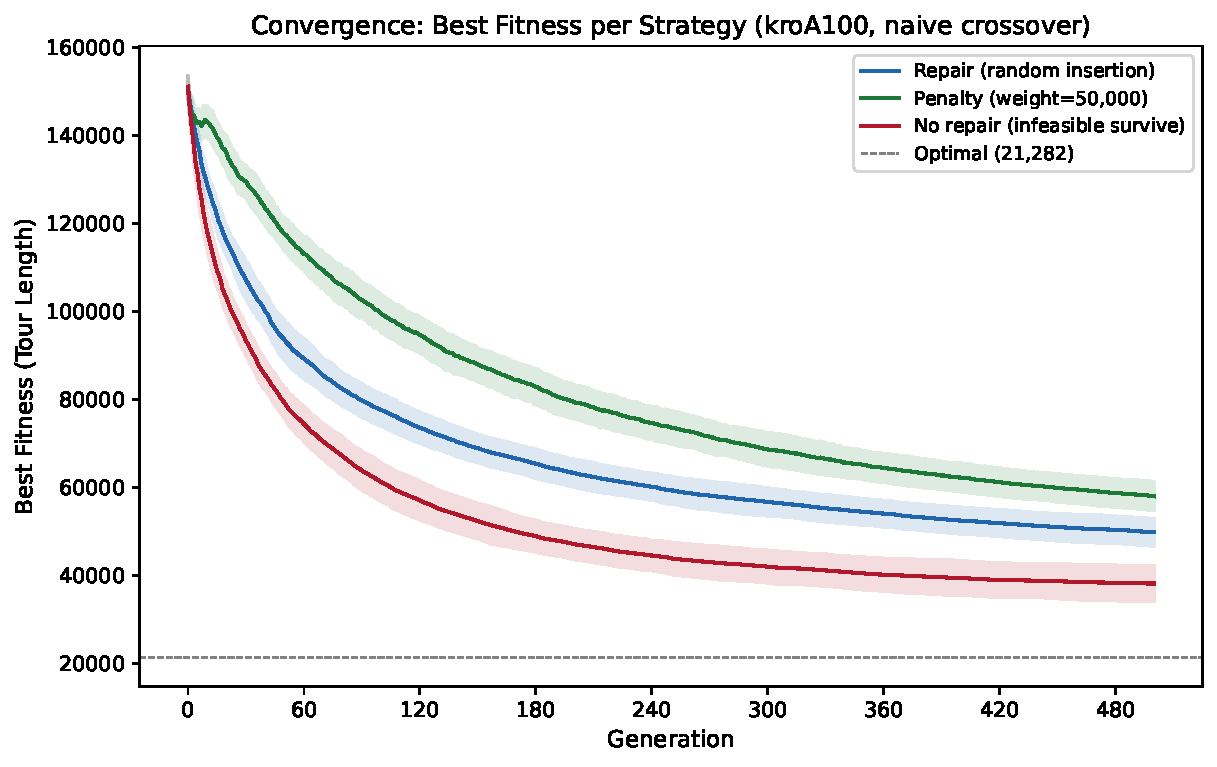
\includegraphics[width=0.85\textwidth]{../results/figures/convergence_best_fitness.pdf}
    \caption{Mean best-fitness convergence per constraint-handling strategy (30 seeds, kroA100). Repair converges to the lowest plateau, PMX overlaps closely, and the penalty arm remains elevated.}
    \label{fig:conv-strategy}
\end{figure}

\fref{fig:conv-combined} adds the mean-population and diversity panels.
All three arms lose the bulk of their population diversity in the first
100 generations. The repair arm retains a marginally higher diversity
floor, likely from the stochastic re-insertion step injecting variation at
repaired loci.

\begin{figure}[htbp]
    \centering
    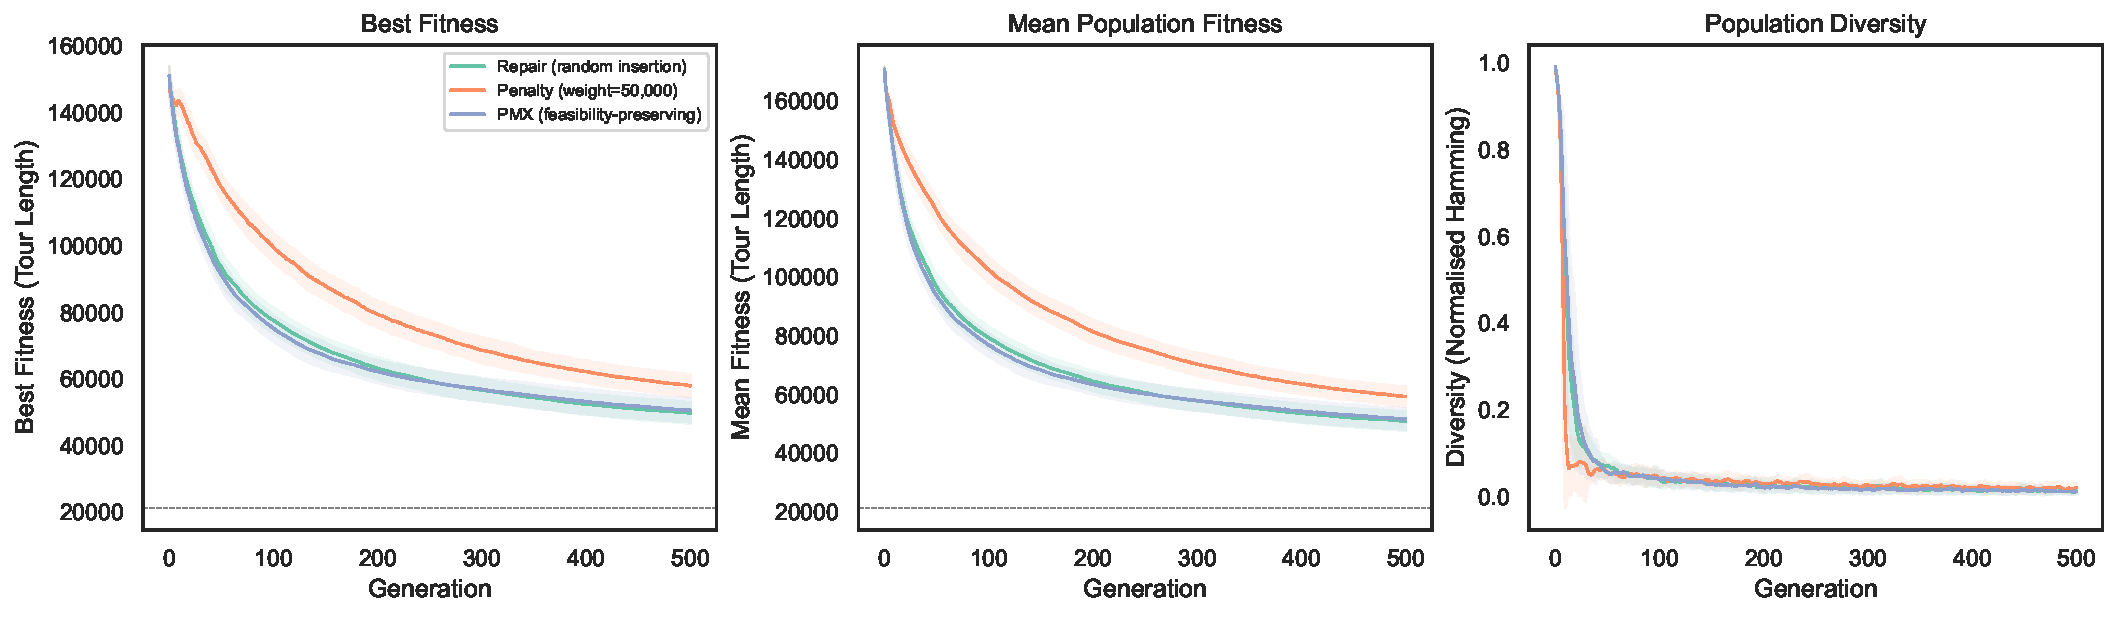
\includegraphics[width=\textwidth]{../results/figures/convergence_combined.pdf}
    \caption{Three-panel convergence: best fitness (left), mean population fitness (centre), and population diversity (right) per strategy.}
    \label{fig:conv-combined}
\end{figure}

The remaining convergence figures isolate each swept parameter, holding the
others at best-configuration values. \fref{fig:conv-pop} shows larger
populations converging to lower final fitness, with diminishing returns past
pop\_size~$=$~200. \fref{fig:conv-mutation} shows the higher mutation rate
($r_m = 0.10$) converging faster and to a lower plateau, while lower rates
stall earlier. \fref{fig:conv-selection} gives the clearest separation:
tournament selection dominates roulette across the full run.

\begin{figure}[htbp]
    \centering
    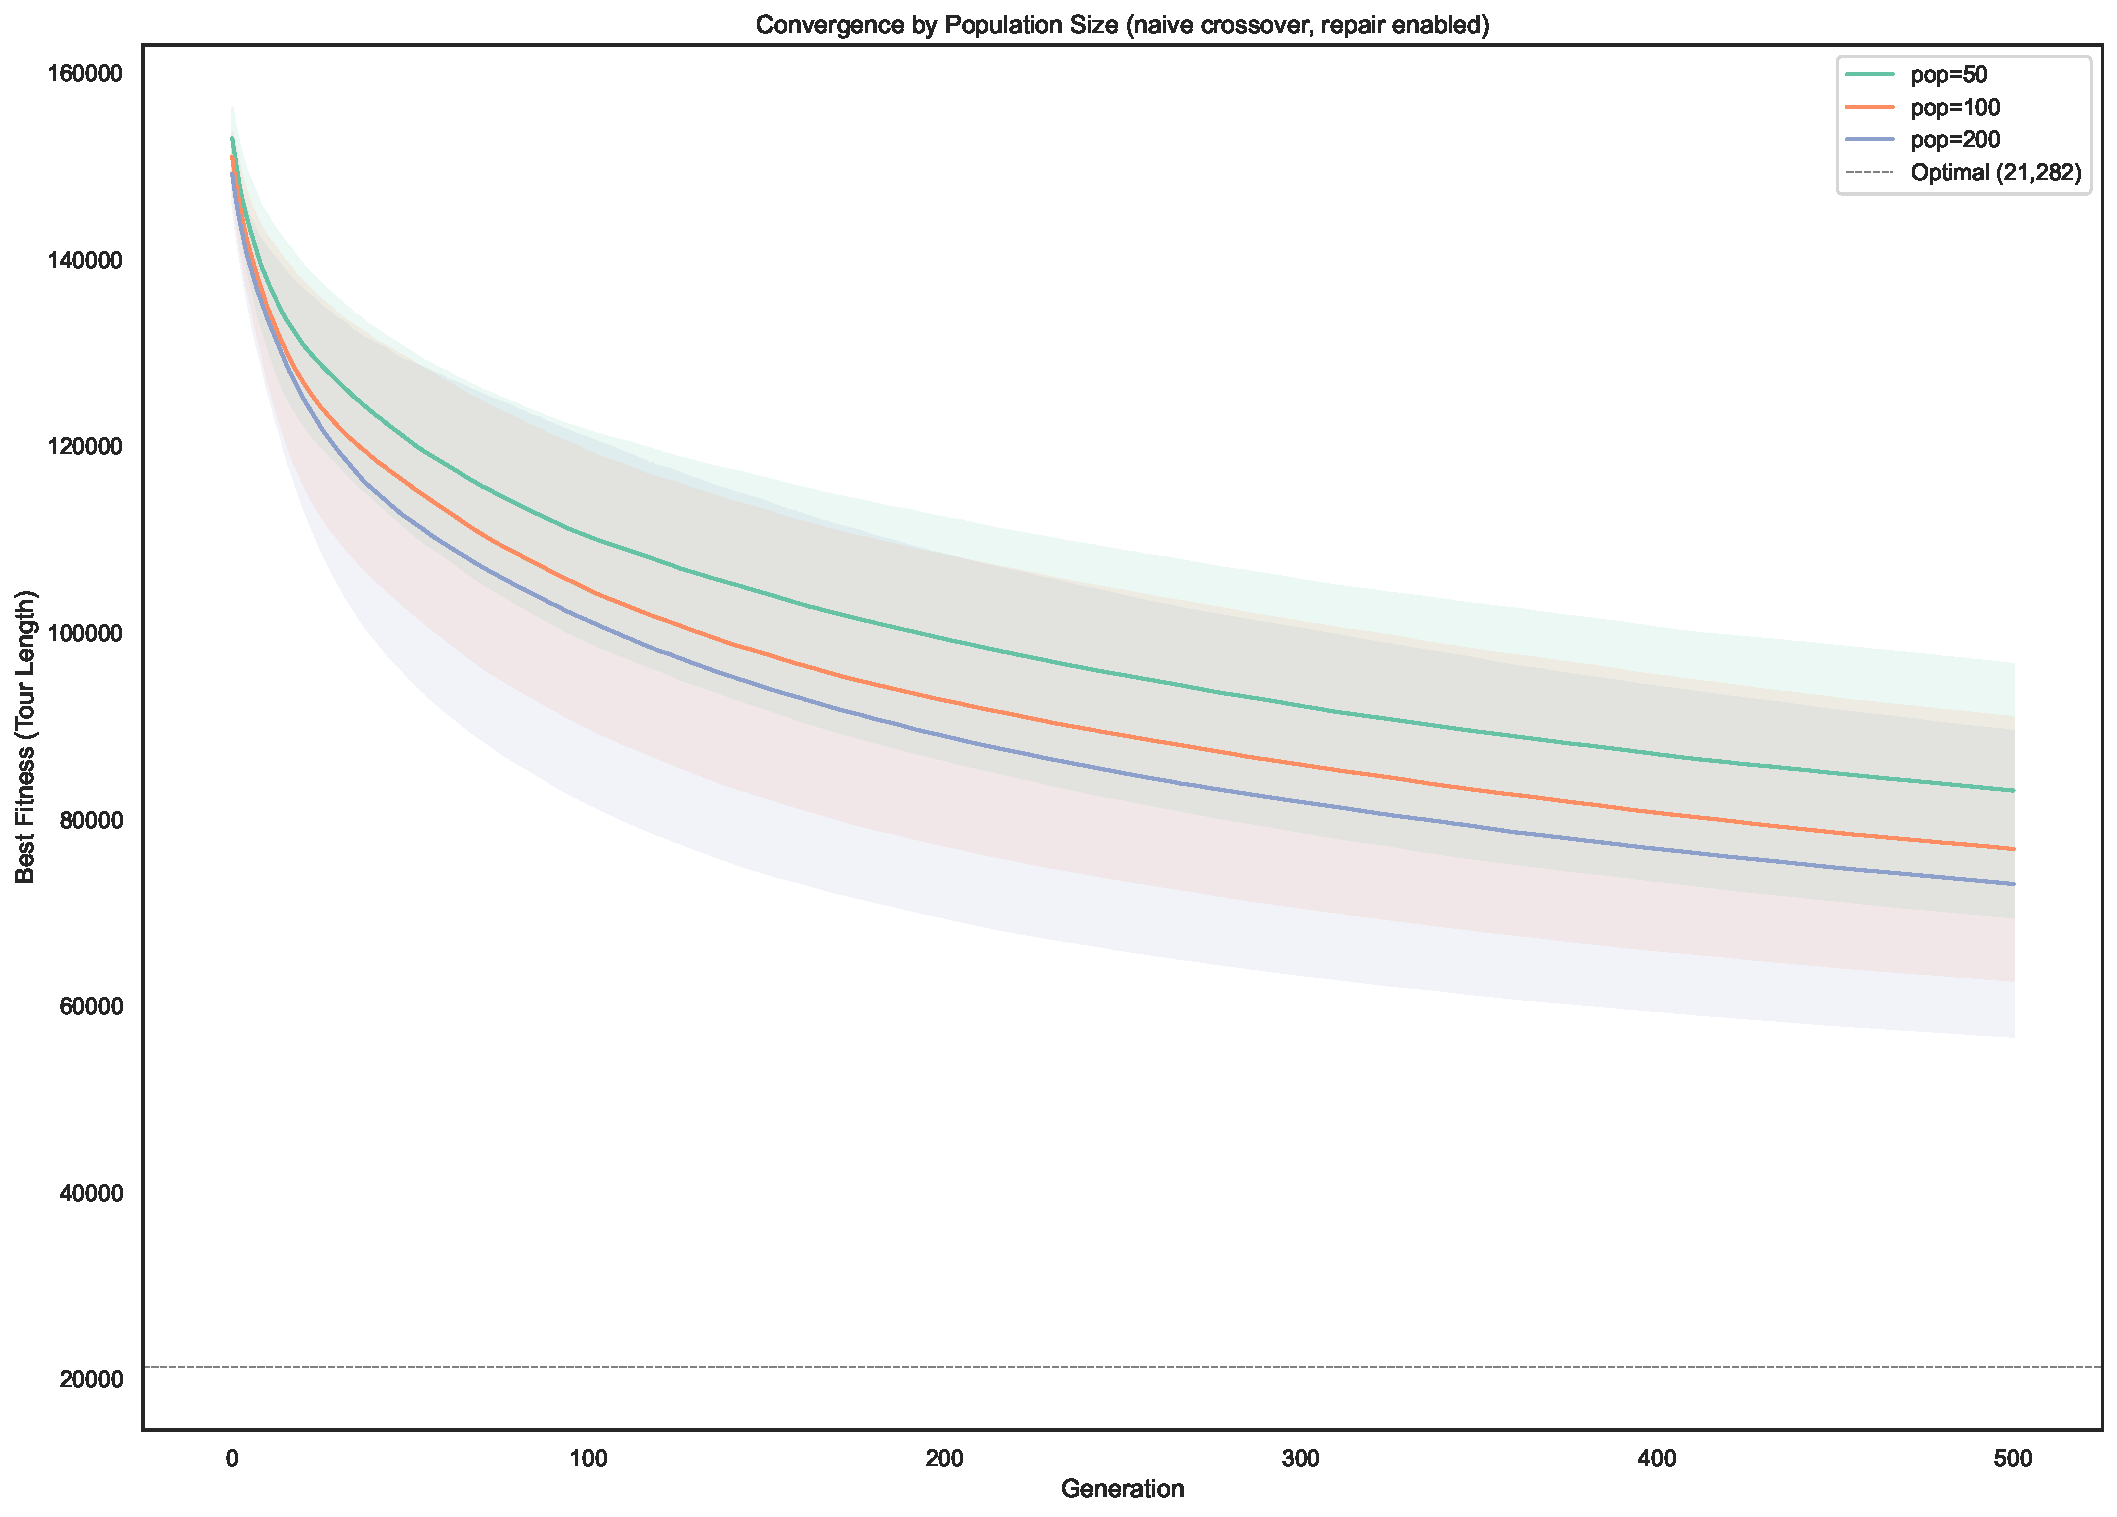
\includegraphics[width=0.85\textwidth]{../results/figures/convergence_by_pop_size.pdf}
    \caption{Best-fitness convergence by population size. Larger populations reach lower plateaus, with diminishing returns past pop\_size~$=$~200.}
    \label{fig:conv-pop}
\end{figure}

\begin{figure}[htbp]
    \centering
    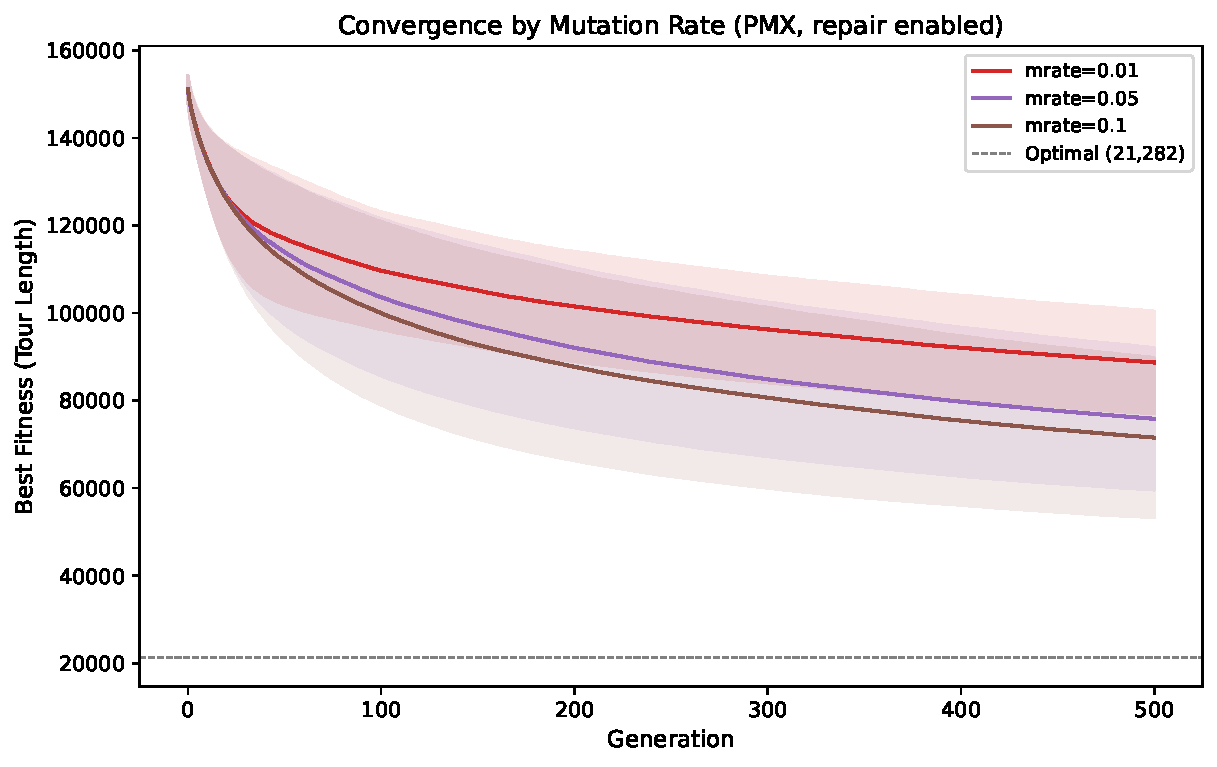
\includegraphics[width=0.85\textwidth]{../results/figures/convergence_by_mutation_rate.pdf}
    \caption{Best-fitness convergence by mutation rate. Higher mutation rates converge faster and to lower final values.}
    \label{fig:conv-mutation}
\end{figure}

\begin{figure}[htbp]
    \centering
    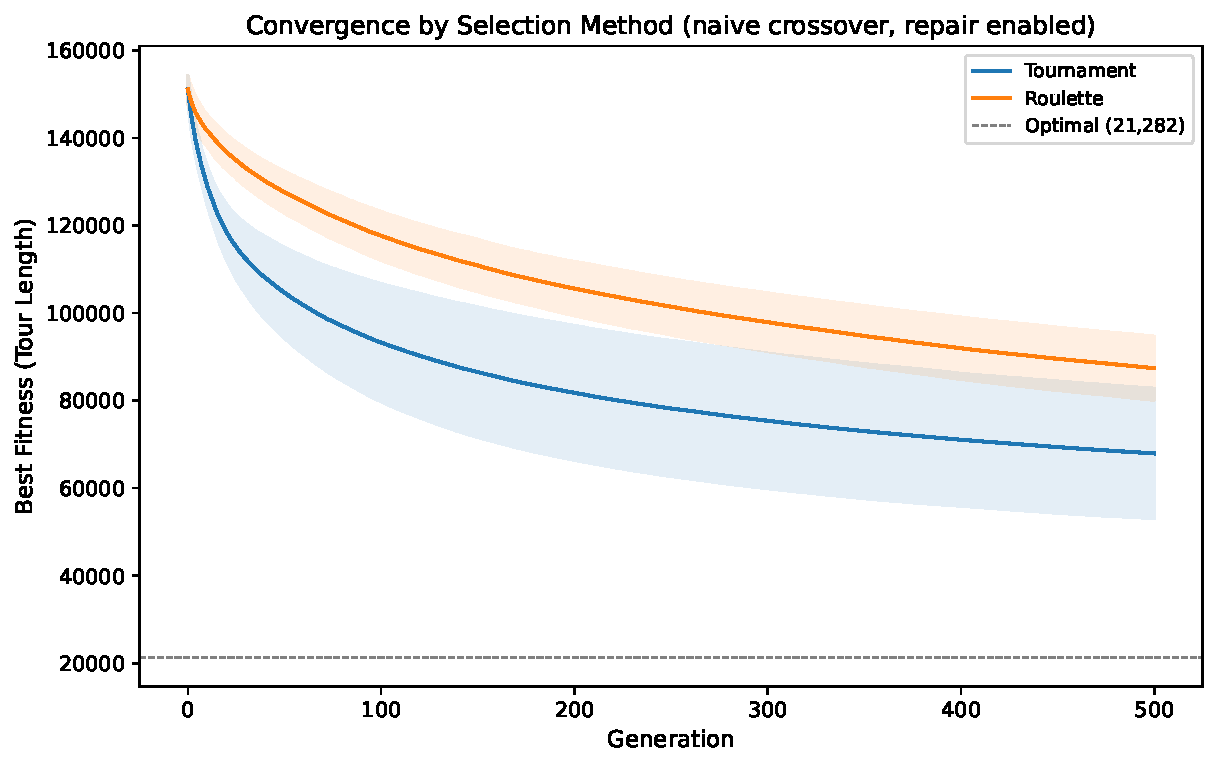
\includegraphics[width=0.85\textwidth]{../results/figures/convergence_by_selection.pdf}
    \caption{Best-fitness convergence by selection method. Tournament selection dominates roulette across the full horizon.}
    \label{fig:conv-selection}
\end{figure}

\fref{fig:conv-best-worst} contrasts the best and worst configurations on a
shared axis. The gap between the two curves is wider than any
single-parameter effect above, which tells us that parameter interactions
matter more than any one parameter alone.

\begin{figure}[htbp]
    \centering
    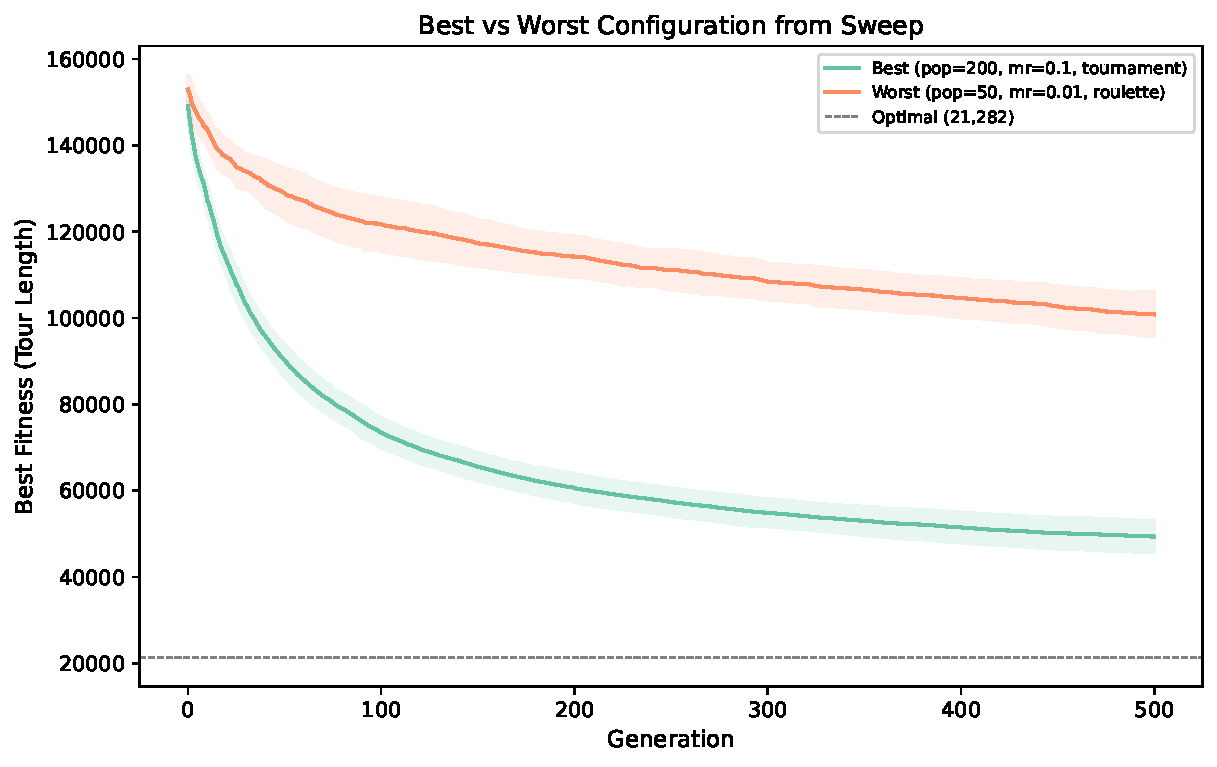
\includegraphics[width=0.85\textwidth]{../results/figures/convergence_best_vs_worst.pdf}
    \caption{Best vs.\ worst sweep configuration. The gap between the two curves exceeds any single-parameter sensitivity, showing that parameter interactions dominate.}
    \label{fig:conv-best-worst}
\end{figure}

\section{Solution-Quality Distribution Across Runs}
\label{T4:Boxplots}

\fref{fig:boxplot-strategy} shows the distribution of final tour lengths for
each constraint-handling arm. All three arms produce valid tours (PMX
preserves the permutation, repair restores it, and the penalty arm resolves
chromosomes to feasibility at evaluation time), so the separation reflects
genuine quality differences. The repair median sits lowest, PMX overlaps
with repair through most of its interquartile range, and the penalty box is
clearly offset above both.

\begin{figure}[htbp]
    \centering
    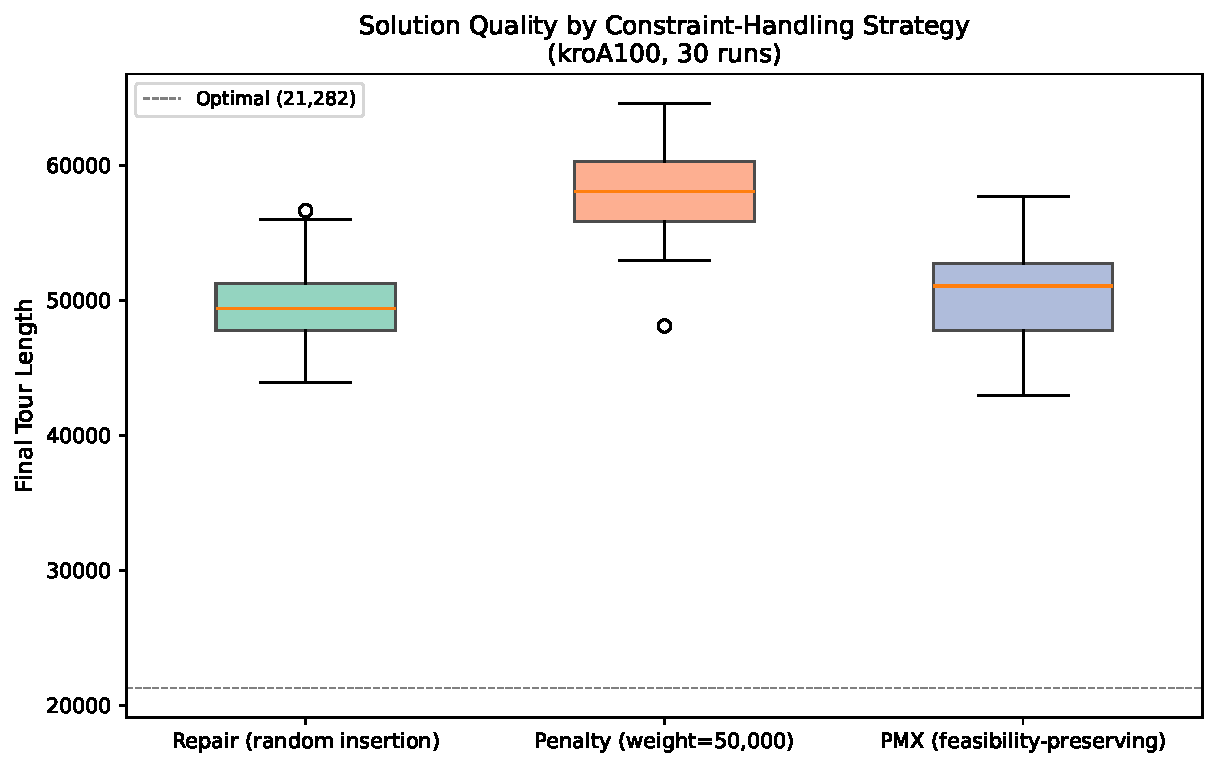
\includegraphics[width=0.8\textwidth]{../results/figures/boxplot_strategy.pdf}
    \caption{Final tour length by constraint-handling strategy (30 runs each). Repair and PMX overlap; penalty is visibly separated upward.}
    \label{fig:boxplot-strategy}
\end{figure}

The per-parameter boxplots in
\fref{fig:boxplot-pop}--\fref{fig:boxplot-selection} mirror the sensitivity
ordering from the convergence curves. Selection method produces the largest
separation --- tournament and roulette do not overlap at all. Mutation rate
shows a monotonic improvement from 0.01 to 0.10. Population size produces a
more modest shift.

\begin{figure}[htbp]
    \centering
    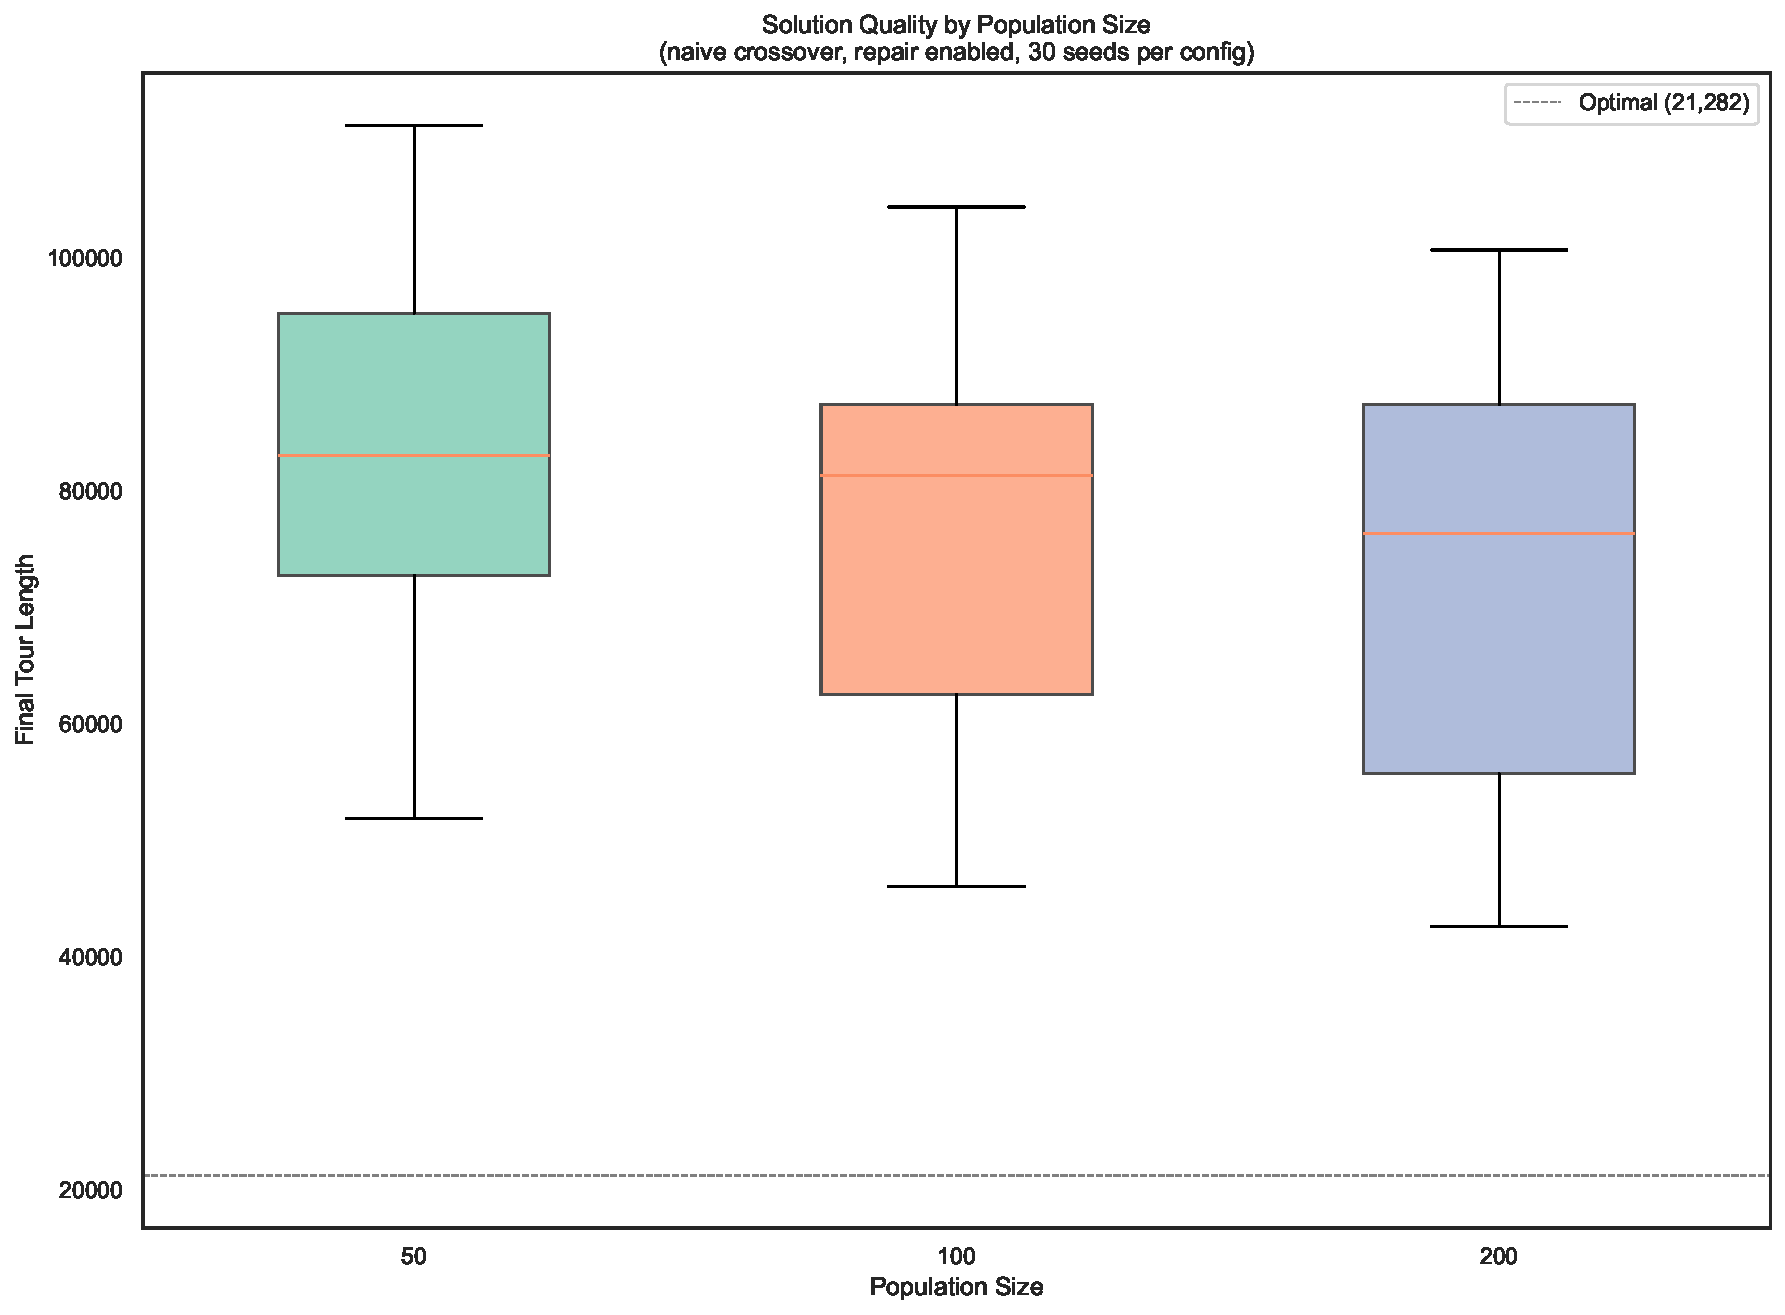
\includegraphics[width=0.8\textwidth]{../results/figures/boxplot_pop_size.pdf}
    \caption{Final tour length by population size. Larger populations produce lower and tighter distributions, but the effect is modest compared to the other two parameters.}
    \label{fig:boxplot-pop}
\end{figure}

\begin{figure}[htbp]
    \centering
    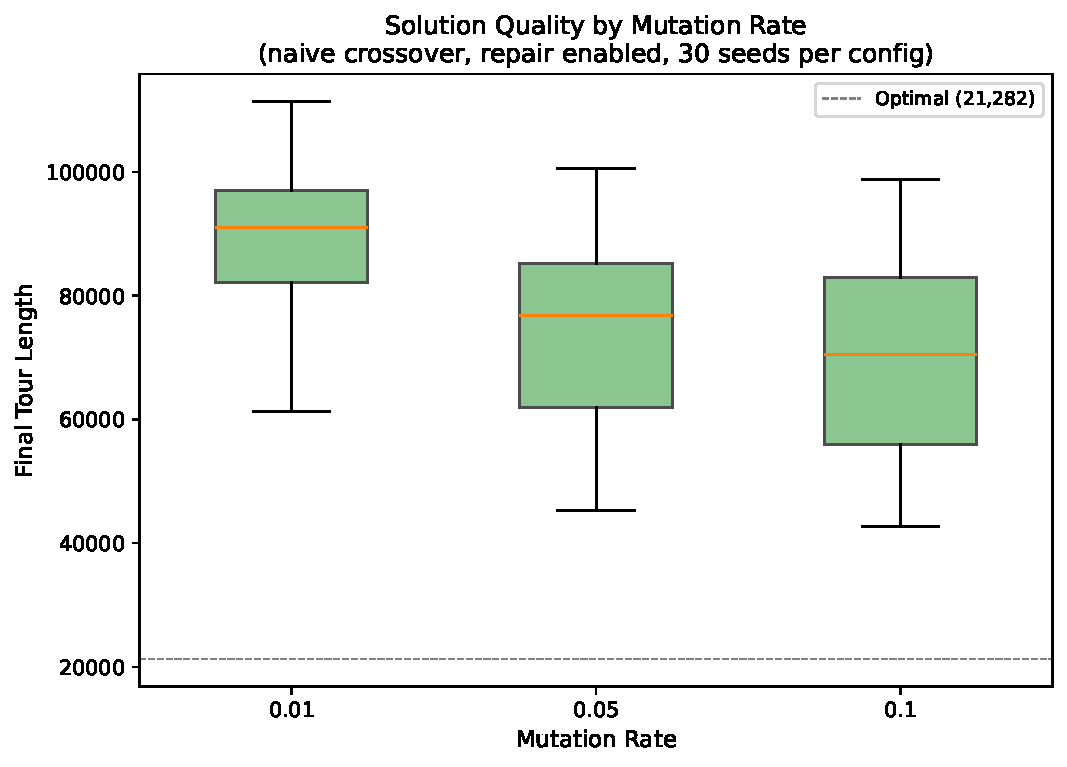
\includegraphics[width=0.8\textwidth]{../results/figures/boxplot_mutation_rate.pdf}
    \caption{Final tour length by mutation rate. A clear monotonic improvement is visible from $r_m = 0.01$ to $r_m = 0.10$.}
    \label{fig:boxplot-mutation}
\end{figure}

\begin{figure}[htbp]
    \centering
    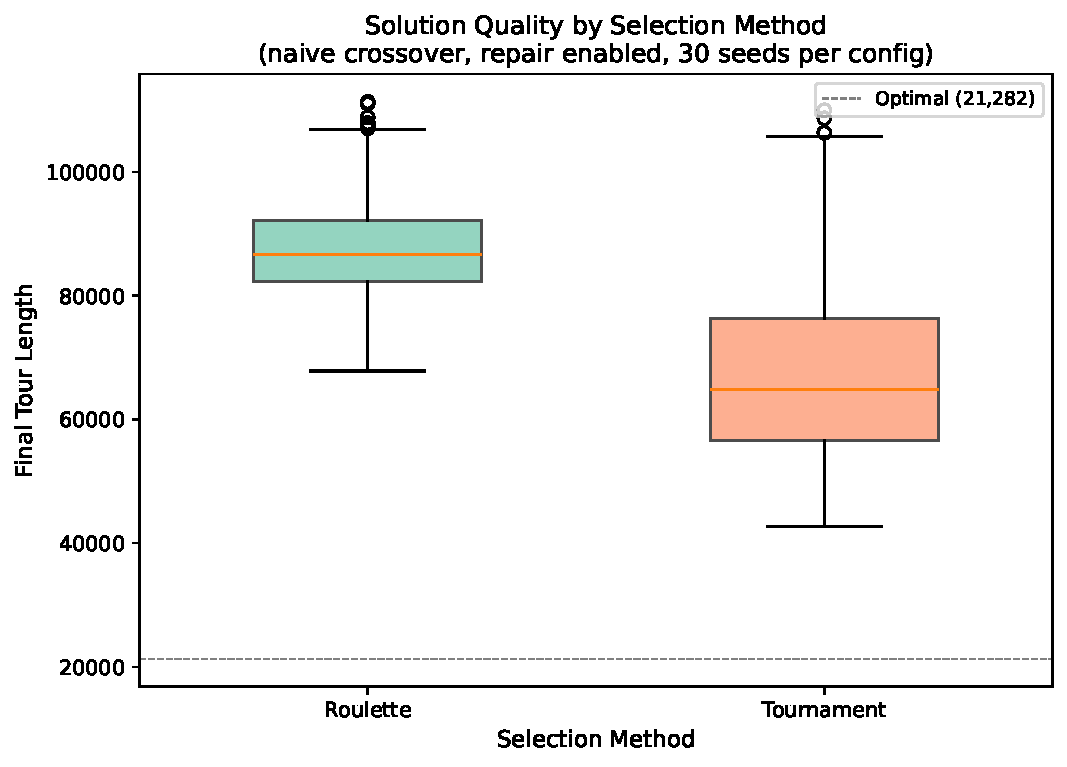
\includegraphics[width=0.8\textwidth]{../results/figures/boxplot_selection_method.pdf}
    \caption{Final tour length by selection method. The tournament and roulette boxes do not overlap, making selection the most influential single parameter.}
    \label{fig:boxplot-selection}
\end{figure}

\section{Best-Tour Visualisation}
\label{T4:BestTour}

\fref{fig:best-tour} renders the best tour found across the entire sweep:
fitness 42{,}622.53, obtained from seed 16 of the best configuration
(pop\_size~$=$~200, $r_c = 0.95$, $r_m = 0.10$, tournament, PMX with
repair). Each edge is drawn with \texttt{matplotlib.pyplot.quiver} so that
the arrowhead shows traversal direction. The gap from the known optimal of
21{,}282 is approximately 100.3\%.

\begin{figure}[htbp]
    \centering
    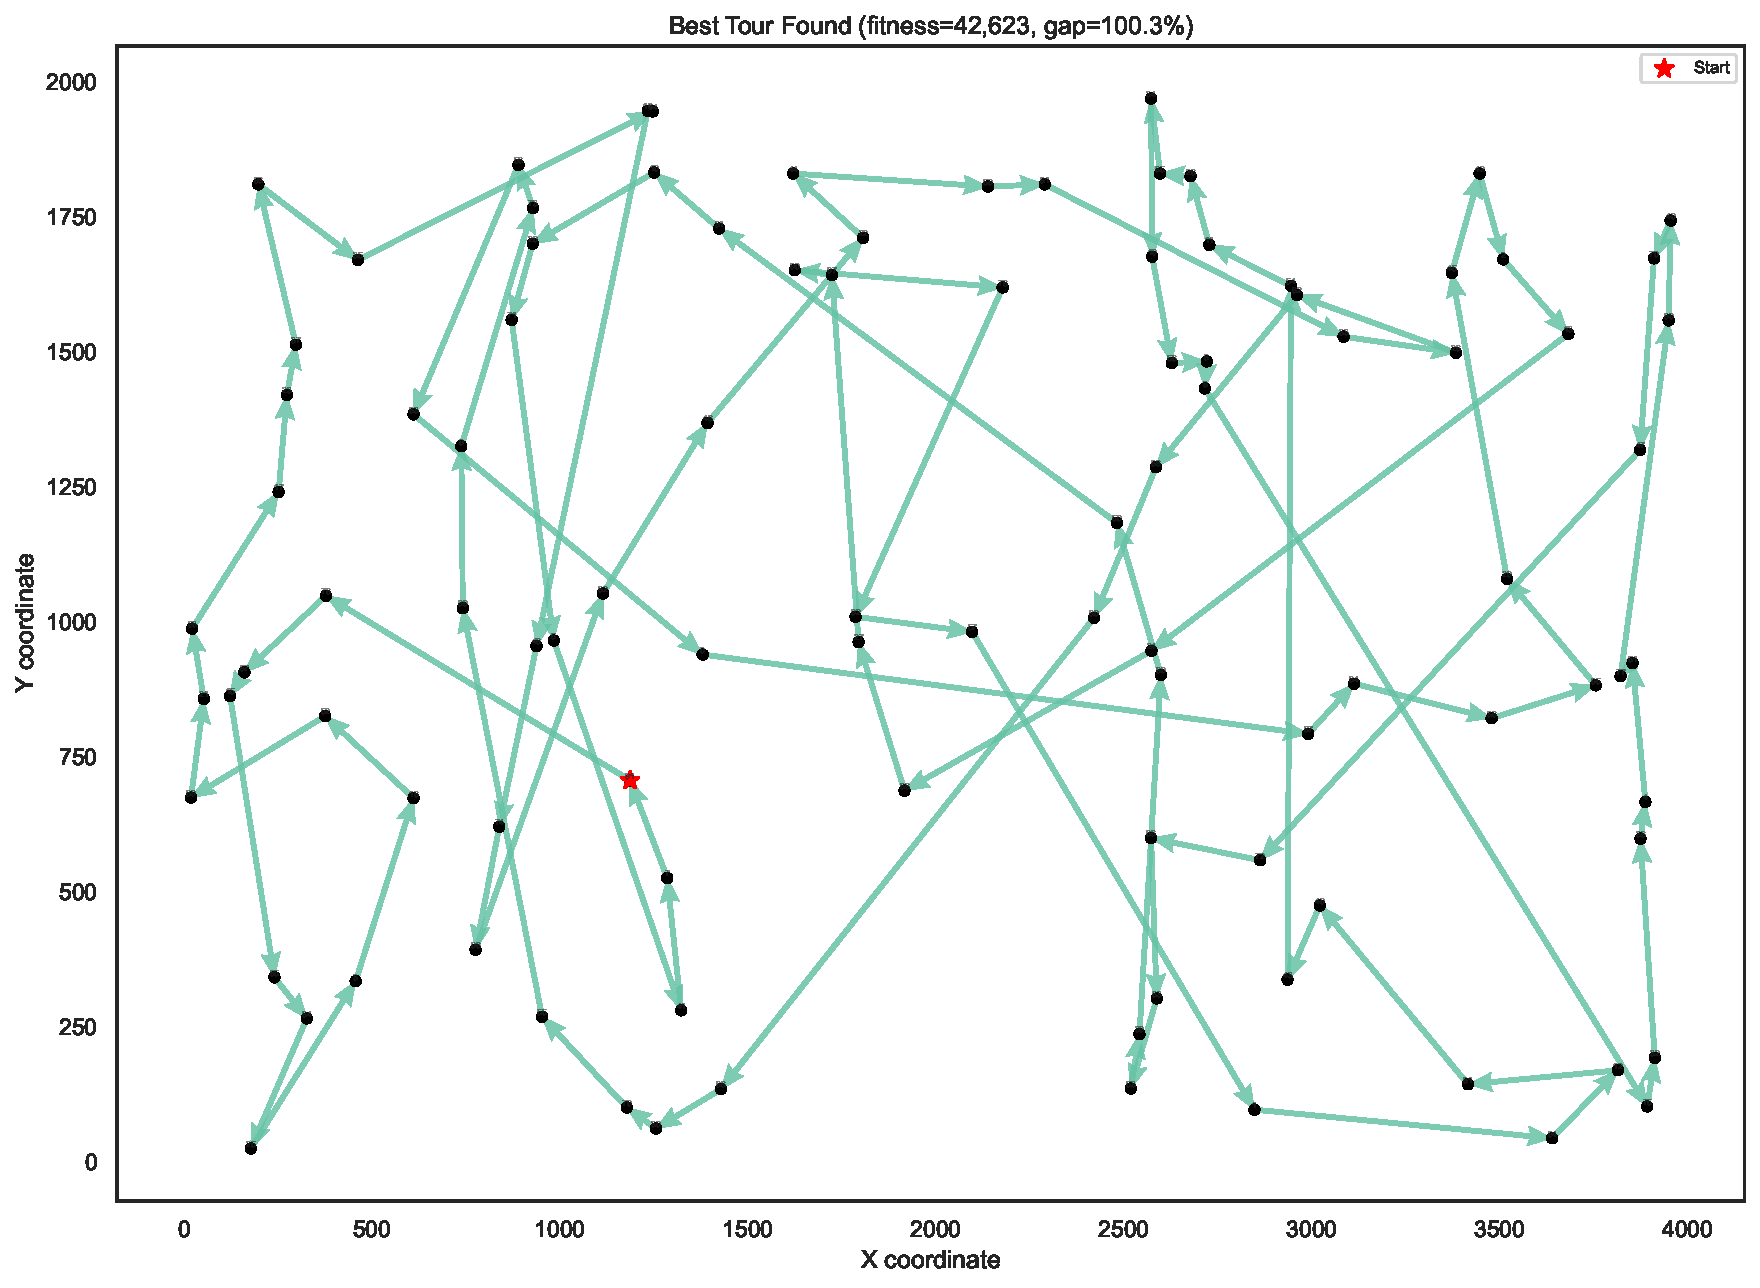
\includegraphics[width=0.75\textwidth]{../results/figures/best_tour.pdf}
    \caption{Best tour found on kroA100 (fitness 42{,}622.53, seed 16, best sweep configuration). Arrows drawn with \texttt{ax.quiver} show traversal direction; the gap from the optimal is 100.3\%.}
    \label{fig:best-tour}
\end{figure}

The large gap is expected. We used naive crossover with random-insertion
repair and no local search; state-of-the-art solvers attach a 2-opt or
Lin--Kernighan step that removes exactly the kind of crossing edges visible
in the figure. Several edges cross and several others detour through a city
that a single 2-opt swap would fix. We are evaluating the assignment's
specified baseline, not a competitive TSP heuristic, and the gap should be
read accordingly.

\section{Results Discussion}
\label{T4:Discussion}

Looking at the results together, the three constraint-handling strategies
rank by mean solution quality as repair $\le$ PMX $<$ penalty.
\fref{fig:boxplot-strategy} fixes this ranking on final tour length, and
\fref{fig:conv-strategy} confirms it is not just a matter of slow
convergence --- the penalty arm plateaus higher rather than catching up.
This aligns with the critique in \sref{T3:RepairCritique}: enforcing
feasibility directly through repair gives the GA a cleaner search signal
than penalising infeasibility.

The per-parameter views in
\fref{fig:conv-pop}--\fref{fig:conv-selection} and
\fref{fig:boxplot-pop}--\fref{fig:boxplot-selection} agree on the same
influence ranking: selection method first, mutation rate second, population
size third. The best-vs-worst gap in \fref{fig:conv-best-worst} exceeds any
single-parameter effect, which means these parameters interact rather than
acting additively.

The absolute gap from optimal is the obvious limitation. As we noted in
\sref{T3:RepairCritique} and as \fref{fig:best-tour} makes visible, the
residual crossings would yield to a 2-opt local search applied inside the
GA loop or as a post-processing step. That is the most direct extension of
this work, and it would close the gap without changing the
constraint-handling conclusions.
